% !TEX root = ../bachlor-arbeit.tex
The $S$-matrix calculus enables us to calculate the optical behavior of a stack if we know the optical behavior of all its layers in the form of their $S$-matrices. In section \ref{sec:s_mats} we derived the $S$-matrices of propagation through and interfaces between homogeneous isotropic materials. This calculation is based on the Fresnel equations and is therefore analytic. However we cannot calculate the $S$-matrix of a metasurface analytically. This results in a semi-analytic Stacking Algorithm where the $S$-matrices of the metasurfaces need to be provided but the remaining $S$-matrices can be calculated based on geometric parameters.
\\


$\qquad$ A core idea of this algorithm is the fact that geometric transformations like rotation and mirroring can be applied directly to Jones matrices. For example let $\hat M$ be the Jones matrix of an optical component then the Jones matrix of the rotated component $\hat{M}_{\varphi}$ is calculated as:

\begin{equation}
    \hat{M}_{\varphi} = \hat \Theta(-\varphi) \, \hat{M} \, \hat \Theta(\varphi)
    \qq{where}
    \hat \Theta(\varphi) =
    \begin{pmatrix}
        \cos \varphi & \sin \varphi \\
        -\sin \varphi & \cos \varphi
    \end{pmatrix}
\end{equation}

On this basis we can rotate $S$-matrices in a similar manner:

\begin{equation}
    \hat S_\varphi =
    \begingroup
    \renewcommand*{\arraystretch}{1.5}
        \begin{pmatrix}
            \hat \Theta(-\varphi) \hat T^f \hat \Theta(\varphi)&
            \hat \Theta(-\varphi) \hat R^b \hat \Theta(\varphi)\\
            \hat \Theta(-\varphi) \hat R^f \hat \Theta(\varphi)&
            \hat \Theta(-\varphi) \hat T^b \hat \Theta(\varphi)
        \end{pmatrix}
    \endgroup
\end{equation}

Flipping and mirroring of $S$-matrices is done analogously. With all mathematical operations well defined we can write down SASA in pseudo code.

\comment{
\begin{figure}[H]
    \centering
    \includegraphics[width=.4\linewidth]{bg_two_layers}
    \caption{An example for a two layer metasurface stack. The top layer consist of rectangular gold particles arranged on a square matrix of period $\Lambda$. The bottom layer consist of rectangular holes in a gold sheet which are rotated by an angle of $\varphi$ in respect to the top layer. The two metasurfaces are separated by a glass spacer of thickness $d$.}
    \label{fig:bg:two_layers}
\end{figure}
}

\begin{figure}[H]
\begin{algorithm}[H]
    \SetAlgoLined
    \KwIn{Stack = $[\text{Layer}\, 0, \, \text{Layer 1}, \, \, \dots]$}
    \KwOut{Stack $S$-matrix}
    $S$-mats = $[\ ]$ \\
    \For{$i = 0$;  $i < \s{len}(\s{Stack})$;  $i = i+1$;}{
        \uIf{Stack$[i]$ \KwIs metasurface}{
            add layer $\hat S$ to $S$-mats
        } \Else {
            calculate propagation $S$-matrix $\hat S_{n_i,d_i}$ \\
            add $\hat S_{n_i,d_i}$ to $S$-mats
        }
        apply geometric transformations to added $S$-matrix \\
        calculate interface $S$-matrix $\hat S_{n_i,n_{i+1}}$ \\
        add $\hat S_{n_i,n_{i+1}}$ to $S$-mats
    }
    $\hat S = \mathds 1$ \\
    \For{$i = 0$;  $i < \s{len}(\text{S-mats})$;  $i = i+1$;}{
        $\hat S = \hat S \star S$-mats$[i]$
    }
    \KwRet{$\hat S$}
\end{algorithm}
\begin{tabular}{ll}
    SASA pseudo code: &
    \begin{tabular}[t]{@{}l@{}}
        A Layer variable holds all the information of that layer, that is the $S$-matrix if \\
        its a metasurface and the refractive index $n$ and thickness $d$ otherwise.
    \end{tabular}\\
\end{tabular}
\end{figure}


\paragraph{Conditions}~\\
\label{par:conditions}For this algorithm to produce physical valid output some conditions need to be met. Equations that are boundary conditions to the algorithm will be marked bold. It has been shown \note{needs cite} that the $S$-matrix calculus can only be used when the meta materials in the stack do not interact with each other via the near field. That is, only the zeroth diffraction order of a metasurface can be non-evanescent and higher orders need to have decayed enough when they reach the next metasurface.


First we need to ensure that only the zeroth diffraction order is non evanescent by requiring

\begin{boldequation} \label{bg:eq:lamda}
    \lambda > \max(n^f, n^b) \cdot \Lambda
\end{boldequation}

Additionally the distance between metasurfaces needs to be large enough so that all higher order modes have decayed. It was shown in \cite{Menzel2016} that if we demand

\begin{boldequation}
    e^{\Im(k_z)d} < e^{-2} \approx 0.14 \qq{then}
    d > \frac{\Lambda}{\pi \sqrt{1 - \frac{\Lambda^2 n^2}{\lambda^2}}}
\end{boldequation}

The factor $e^{-2}$ was chosen arbitrarily. A smaller value increases the agreement of the $S$-matrix calculus and more rigorous numerical methods which also take into account the near field. One of these, the \hyperref[sec:FMM]{Fourier Modal Method} will be described in more detail in section \ref{sec:opt}.

\paragraph{Symmetries}~\\
\label{sec:symmetries}We can use geometric transformations to examine the $S$-matrices of metasurfaces which satisfy certain symmetries. Lets start with mirror symmetry. The Jones matrix $\hat M'$ of a mirrored component $\hat M$ can be calculated as

\begin{equation}
    \hat M' = \hat F^{-1} \hat M \hat F \qq{where}
    \hat F =
    \begin{pmatrix}
        1 & \phantom{-} 0 \\
        0 & -           1
    \end{pmatrix}
\end{equation}

If a metasurface has mirror symmetry the $S$-matrix needs to satisfy
$\hat S = \hat S'$
and that means all the contained Jones matrices need to satisfy the condition too

\begin{equation}
\begin{aligned}
    \qq*{Let} \hat T^f =
    &\begin{pmatrix}
        A & B \\
        C & D
    \end{pmatrix}
    \qq{then} \\
    \qty(\hat T^f)' =
    \hat F^{-1} \hat T^f \hat F =
    \begin{pmatrix}
        1 & \phantom{-} 0 \\
        0 & -           1
    \end{pmatrix}
    &\begin{pmatrix}
        A & B \\
        C & D
    \end{pmatrix}
    \begin{pmatrix}
        1 & \phantom{-} 0 \\
        0 & -           1
    \end{pmatrix}
    \stackrel{!}{=}
    \begin{pmatrix}
        A & B \\
        C & D
    \end{pmatrix} =
    \hat T^f \\
    \Rightarrow \qquad
    \hat T^f =
    &\begin{pmatrix}
        A & 0 \\
        0 & D
    \end{pmatrix}
\end{aligned}
\end{equation}

We can also examine rotational symmetry with the rotation matrix $\hat \Theta(\varphi)$. A metasurface of $C_4$ symmetry, for example square shaped meta particles, maps onto itself if rotated $90^\circ$. That means the $S$-matrix should also remain equal, so
$\hat S_{\pi/2} \stackrel{!}{=} \hat S$
and

\begin{equation}
\begin{aligned}
    \hat T^f_{\pi/2} =
    \hat \Theta(-\pi/2) \,
    \hat T^f \,
    \hat \Theta(\pi/2)
    &\stackrel{!}{=}
    \hat T^f
    \qq*{,}
    \hat \Theta(\pi/2) =
    \begin{pmatrix}
        \phantom{-} 0 & 1 \\
        -1 & 0
    \end{pmatrix} \\
    \Rightarrow \qquad
    \hat T^f &=
    \begin{pmatrix}
        \phantom{-} A & B \\
        -           B & A
    \end{pmatrix}
\end{aligned}
\end{equation}

So if a metasurface has both mirror and $C_4$ symmetry its $\hat T^f$ matrix has the form

\begin{equation}
    \quad
    \hat T^f =
    \begin{pmatrix}
        A & 0 \\
        0 & A
    \end{pmatrix}
\end{equation}

That means in this case the star product is commutative and the stack will behave the same for light coming from the top and bottom.
And it should be noted that these considerations apply to all Jones matrices and not only to $\hat T^f$.
